\documentclass{article}
\usepackage[utf8]{inputenc}
%\usepackage[english]{babel}
\usepackage[portuguese]{babel}
\usepackage{graphicx}
\usepackage[hidelinks]{hyperref}
\usepackage{amsmath} %lets us use \begin{proof}
%\usepackage[]{amssymb} %gives us the character \varnothing
\usepackage[dvipsnames]{xcolor}
\usepackage{verbatim}

\title{Universidade Federal de Pernambuco \\
Macroeconomia 2 - Lista 5 e 6}
\author{Monitor: Paulo Silva}
\date{11 de novembro de 2022}

\begin{document}
\maketitle %This command prints the title based on information entered above

\section*{Lista 5 - Modelo NK}
\subsection*{Questão 6}
\begin{figure}[!tbh]
    \centering
    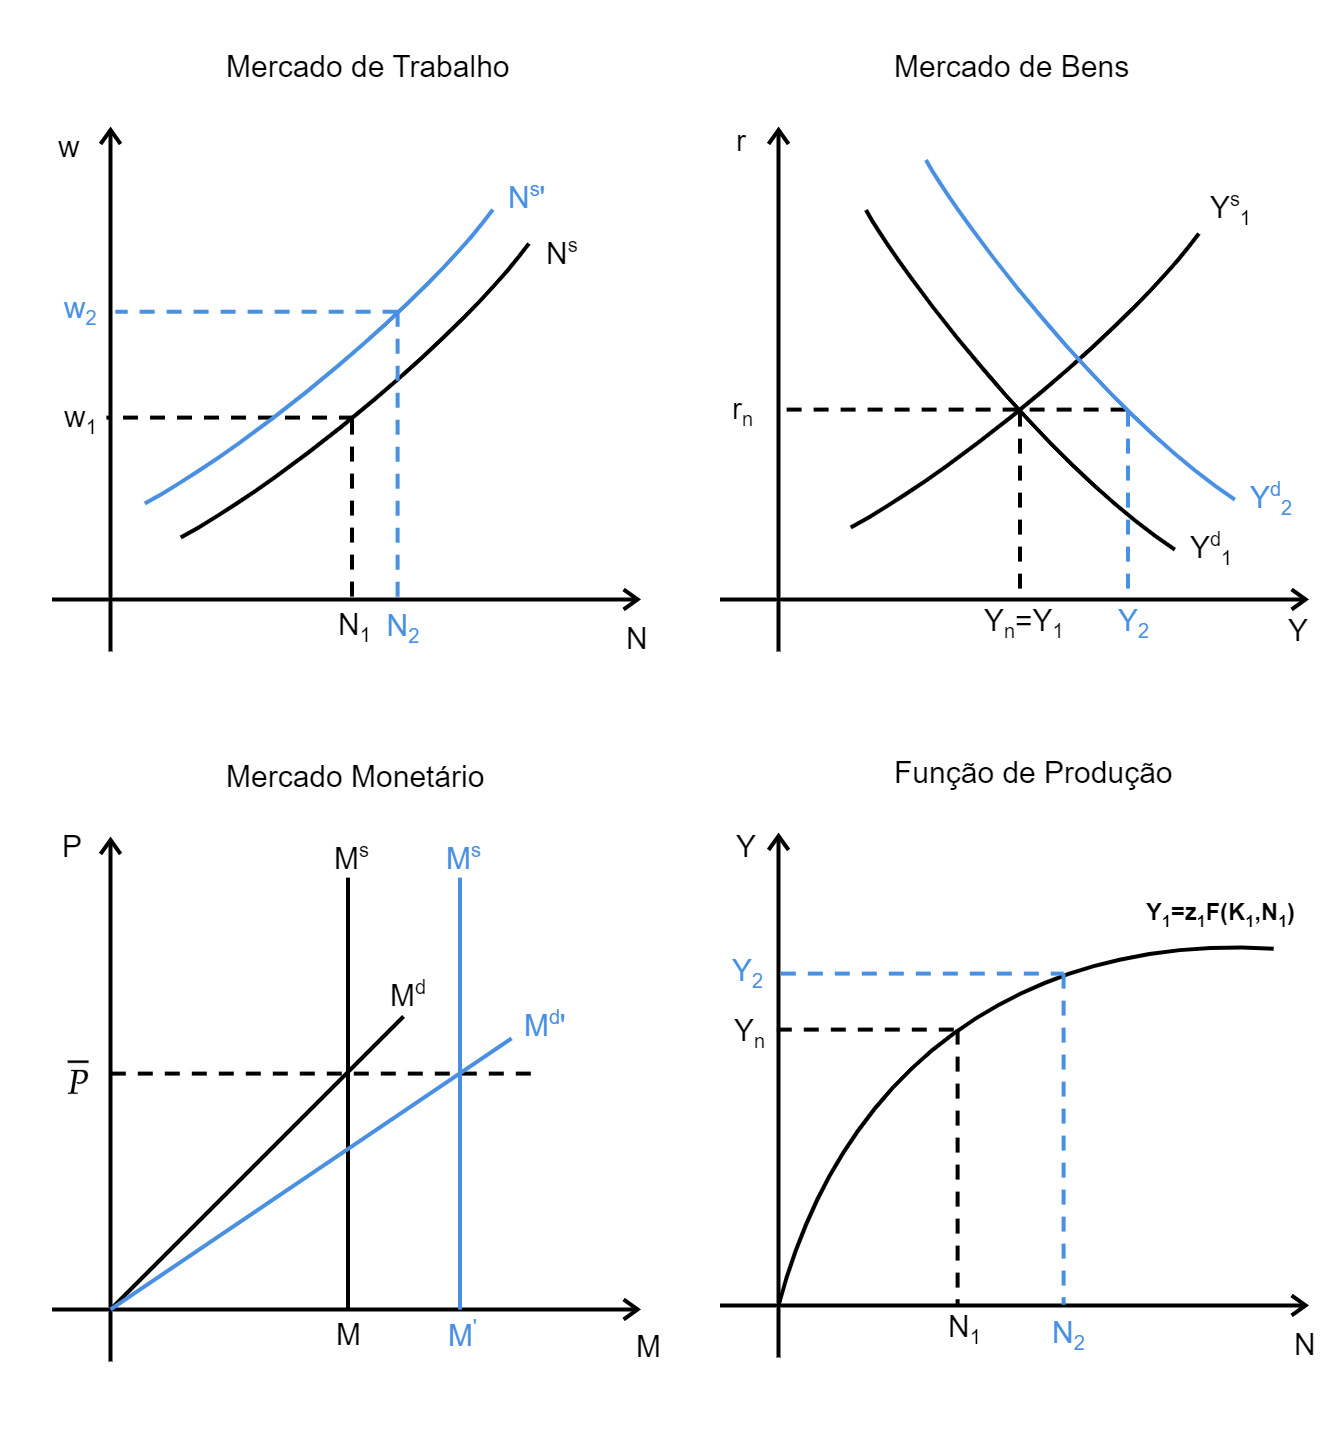
\includegraphics[width=\textwidth]{Q6.png}
    \caption{NK model - Menor prêmio ao risco}
    \label{fig:Q6}
\end{figure}
A taxa de juros enfrentadas pelas famílias e firmas é $r^e=r+s$. \\\\
Uma redução no prêmio de risco (s) incentiva o investimento o que desloca a curva de demanda agregada para a direita com um maior produto (para mesma taxa de juros da economia) demandando um maior nível de trabalho. \\\\
Mas ao mesmo tempo as famílias reduzem a oferta de trabalho (efeito substituição - lazer hoje é mais barato), assim, para uma maior quantidade de trabalho, um maior nível de salário é exigido. \\\\
No mercado monetário, há uma maior demanda por liquidez via aumento do produto, e dado que os preços são rígidos, o banco central deve aumentar a oferta de moeda para manter a meta de juros.\\\\
Graficamente, teremos que:
\clearpage

\section*{Lista 6 - Mundell Fleming (IS-LM-BP)}
\subsection*{Questão 3}
\textbf{Questão: Analisar o efeito nesta economia de um choque negativo (pessimismo das firmas por exemplo, em câmbio flexível). Qual política monetária o banco central deve fazer para manter a taxa de câmbio inalterada? Comparar com cenário inicial.}
\begin{figure}[!tbh]
    \centering
    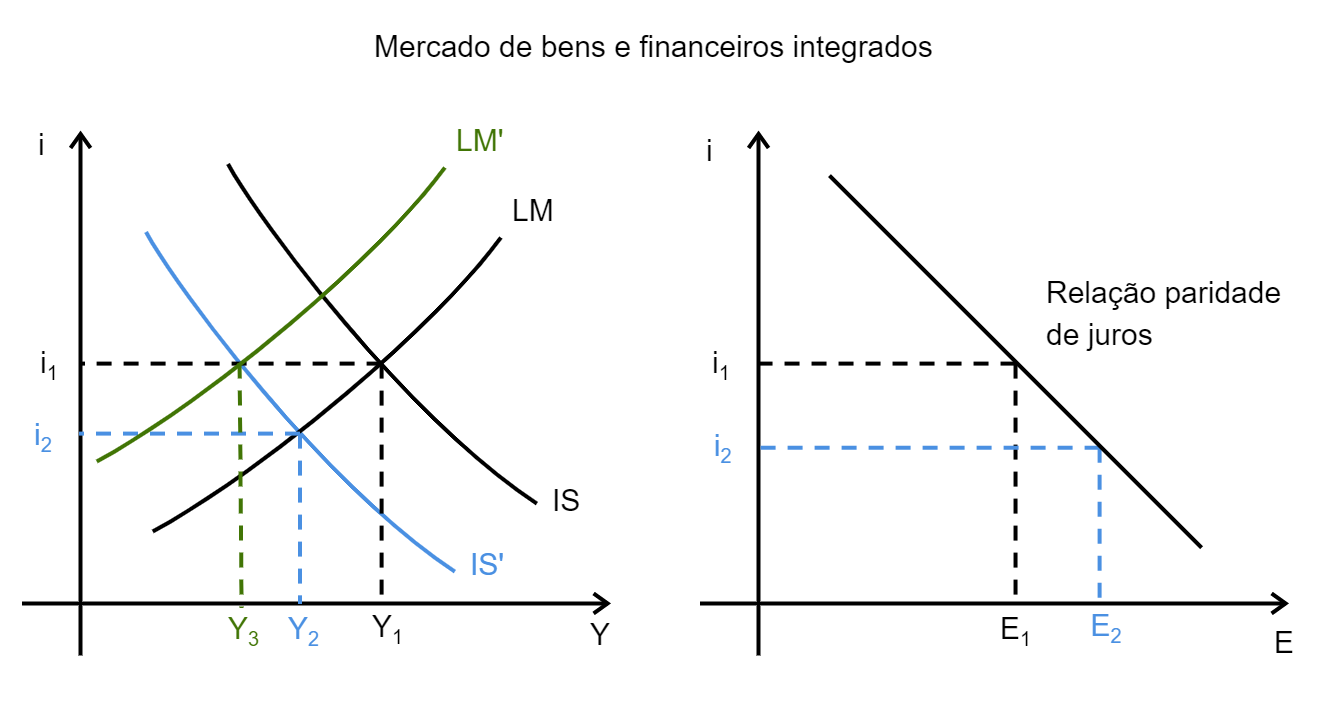
\includegraphics[width=\textwidth]{Q3.png}
    \caption{Mundell Flaming - Choque negativo no mercado de bens}
    \label{fig:Q3}
\end{figure}
\\
Um pessimismo por parte das firmas reduzirá o investimento que retrai a curva IS (pra baixo e esquerda) reduzindo o produto e taxa de juros.\\\\
Com a redução da taxa de juros, a taxa de câmbio aumenta, ou seja, uma depreciação cambial pela relação de paridade de juros.\\\\
Para manter o mesmo nível anterior da taxa de câmbio o banco central pode fazer uma política monetária contracionista elevando a taxa de juros até o nível anterior, ocasionando uma apreciação cambial (queda na taxa de câmbio).\\\\
Comparado a situação inicial, temos um produto menor para a mesma taxa de câmbio e juros observada anteriormente.


\clearpage
\subsection*{Questão 16}
Dados:
$$C=c_0 + c_y Y_d - c_r r^e; \>\>\> r^e=\Bar{r}+x; \>\>\> I=A+i_y Y_d - i_r r^e$$
$$X=\alpha_0+\alpha_1 Y^* + \alpha_2 \epsilon; \>\>\> IM=\theta_0+\theta_1 Y_d - \theta_2 \epsilon; \>\>\> \epsilon=\frac{(1+r^*)}{(1\Bar{r})}\epsilon^e$$
\subsubsection*{Letra A) Encontrar produto de equilíbrio}
Para encontrar o produto de equilíbrio basta isolar o $Y$ da demanda agregada $Y=C+I+G+X-IM$, assim, dada as equações teremos que:
\begin{equation}
    Y = c_0 + c_y Y_d - c_r r^e + A+i_y Y_d - i_r r^e + G + \alpha_0+\alpha_1 Y^* + \alpha_2 \epsilon - \theta_0-\theta_1 Y_d + \theta_2 \epsilon
\end{equation}
Simplificando e substituindo $Y_d=Y-T$:
\begin{equation*}
    Y = \alpha_0+c_0-\theta_0+A+G+(Y-T)(c_y + i_y-\theta_1)-r^e(c_r+i_r)+\alpha_1 Y^* + \epsilon (\alpha_2+\theta_2)
\end{equation*}
Isolando o produto $(Y)$:
\begin{equation*}
    Y(1-c_y - i_y+\theta_1)= \alpha_0+c_0-\theta_0+A+G-T(c_y + i_y-\theta_1)-r^e(c_r+i_r)+\alpha_1 Y^* + \epsilon (\alpha_2+\theta_2)
\end{equation*}
Substituindo a taxa de juros com incerteza $(r^e)$ e a taxa de câmbio $(\epsilon)$:
\begin{equation*}
    Y= \frac{\alpha_0+c_0-\theta_0+A+G-T(c_y + i_y-\theta_1)-r^e(c_r+i_r)+\alpha_1 Y^* + \epsilon (\alpha_2+\theta_2)}{(1-c_y - i_y+\theta_1)}
\end{equation*}
Encontramos o Y de equilíbrio:
\begin{equation}
    Y_{eq}= \frac{\alpha_0+c_0-\theta_0+A+G-T(c_y + i_y-\theta_1)-(\Bar{r}+x)(c_r+i_r)+\alpha_1 Y^* + \left[\frac{(1+r^*)}{(1+\Bar{r})}\epsilon^e\right](\alpha_2+\theta_2)}{(1-c_y - i_y+\theta_1)}
\end{equation}
\subsubsection*{Letra B) Encontrar os efeitos de um aumento no prêmio de risco} 
A ideia é que em equilíbrio, teremos:
\begin{equation*}
    C=c_0 + c_y Y_{eq} -c_y T - c_r (\Bar{r}+x); 
\end{equation*}
\begin{equation*}
    I=A+i_y Y_{eq}-i_y T - i_r (\Bar{r}+x)
\end{equation*}
\begin{equation*}
    X=\alpha_0+\alpha_1 Y^* + \alpha_2 \epsilon
\end{equation*}
\begin{equation*}
    IM=\theta_0+\theta_1 Y_{eq} - \theta_1 T - \theta_2 \epsilon
\end{equation*}
Dessa forma os efeitos de um aumento do prêmio de risco são:
\begin{equation}
    \frac{\partial Y_{eq}}{\partial x} = -\frac{(c_r+i_r)}{(1-c_y-i_y+\theta_0)} < 0
\end{equation}
\begin{equation}
    \frac{\partial C}{\partial x} = c_y \frac{\partial Y_{eq}}{\partial x} - c_r < 0
\end{equation}
\begin{equation}
    \frac{\partial I}{\partial x} = i_y \frac{\partial Y_{eq}}{\partial x} - i_r < 0
\end{equation}
\begin{equation}
    \frac{\partial X}{\partial x} = 0
\end{equation}
\begin{equation}
    \frac{\partial IM}{\partial x} = \theta_1 \frac{\partial Y_{eq}}{\partial x} < 0
\end{equation}
O aumento do prêmio de risco leva a uma queda no produto de equilíbrio, no consumo, investimentos e importações, porém, não modifica as exportações pois este depende apenas da taxa de câmbio (que não foi alterada) e da demanda externa.

\end{document}